We developed the system as a web application using both server-side and client-side programming. This chapter presents both sides of the programming, starting with describing the adjustments made to the design based on findings from Study II. Security considerations and implementation are described at the end of the chapter. The developed application can be found on attached CD. 

\section{Design Changes}

\begin{figure}[h]
  \centering
  \begin{minipage}[b]{0.45\textwidth}
    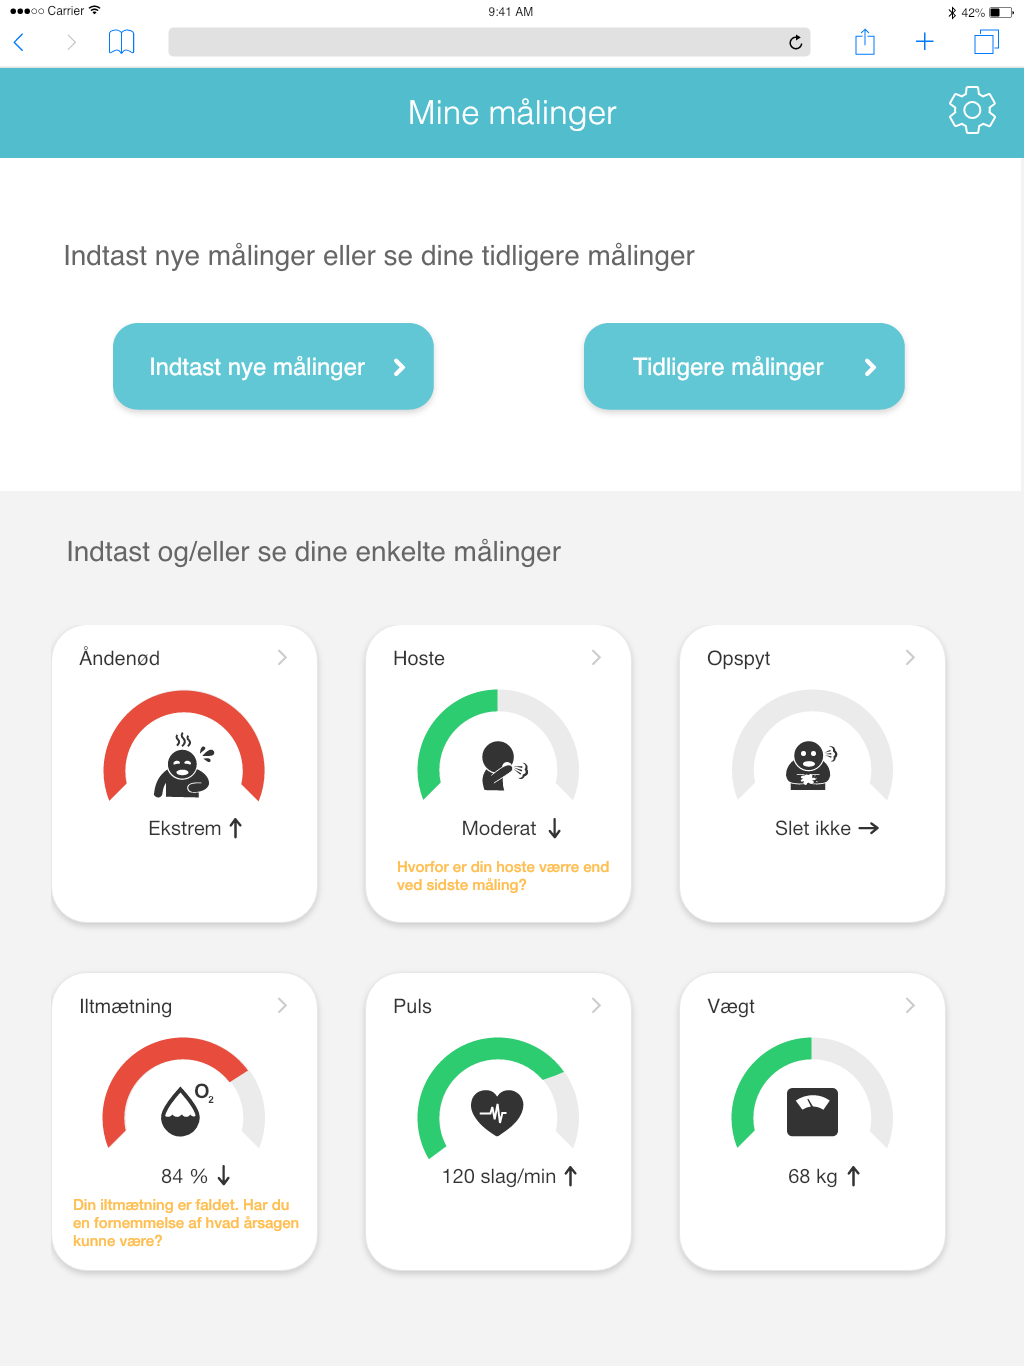
\includegraphics[width=\textwidth]{images/study2/Dashboard.png}
    \caption{Dashboard used in Study II}
    \label{fig:db1st}
  \end{minipage}
  \hfill
  \begin{minipage}[b]{0.45\textwidth}
    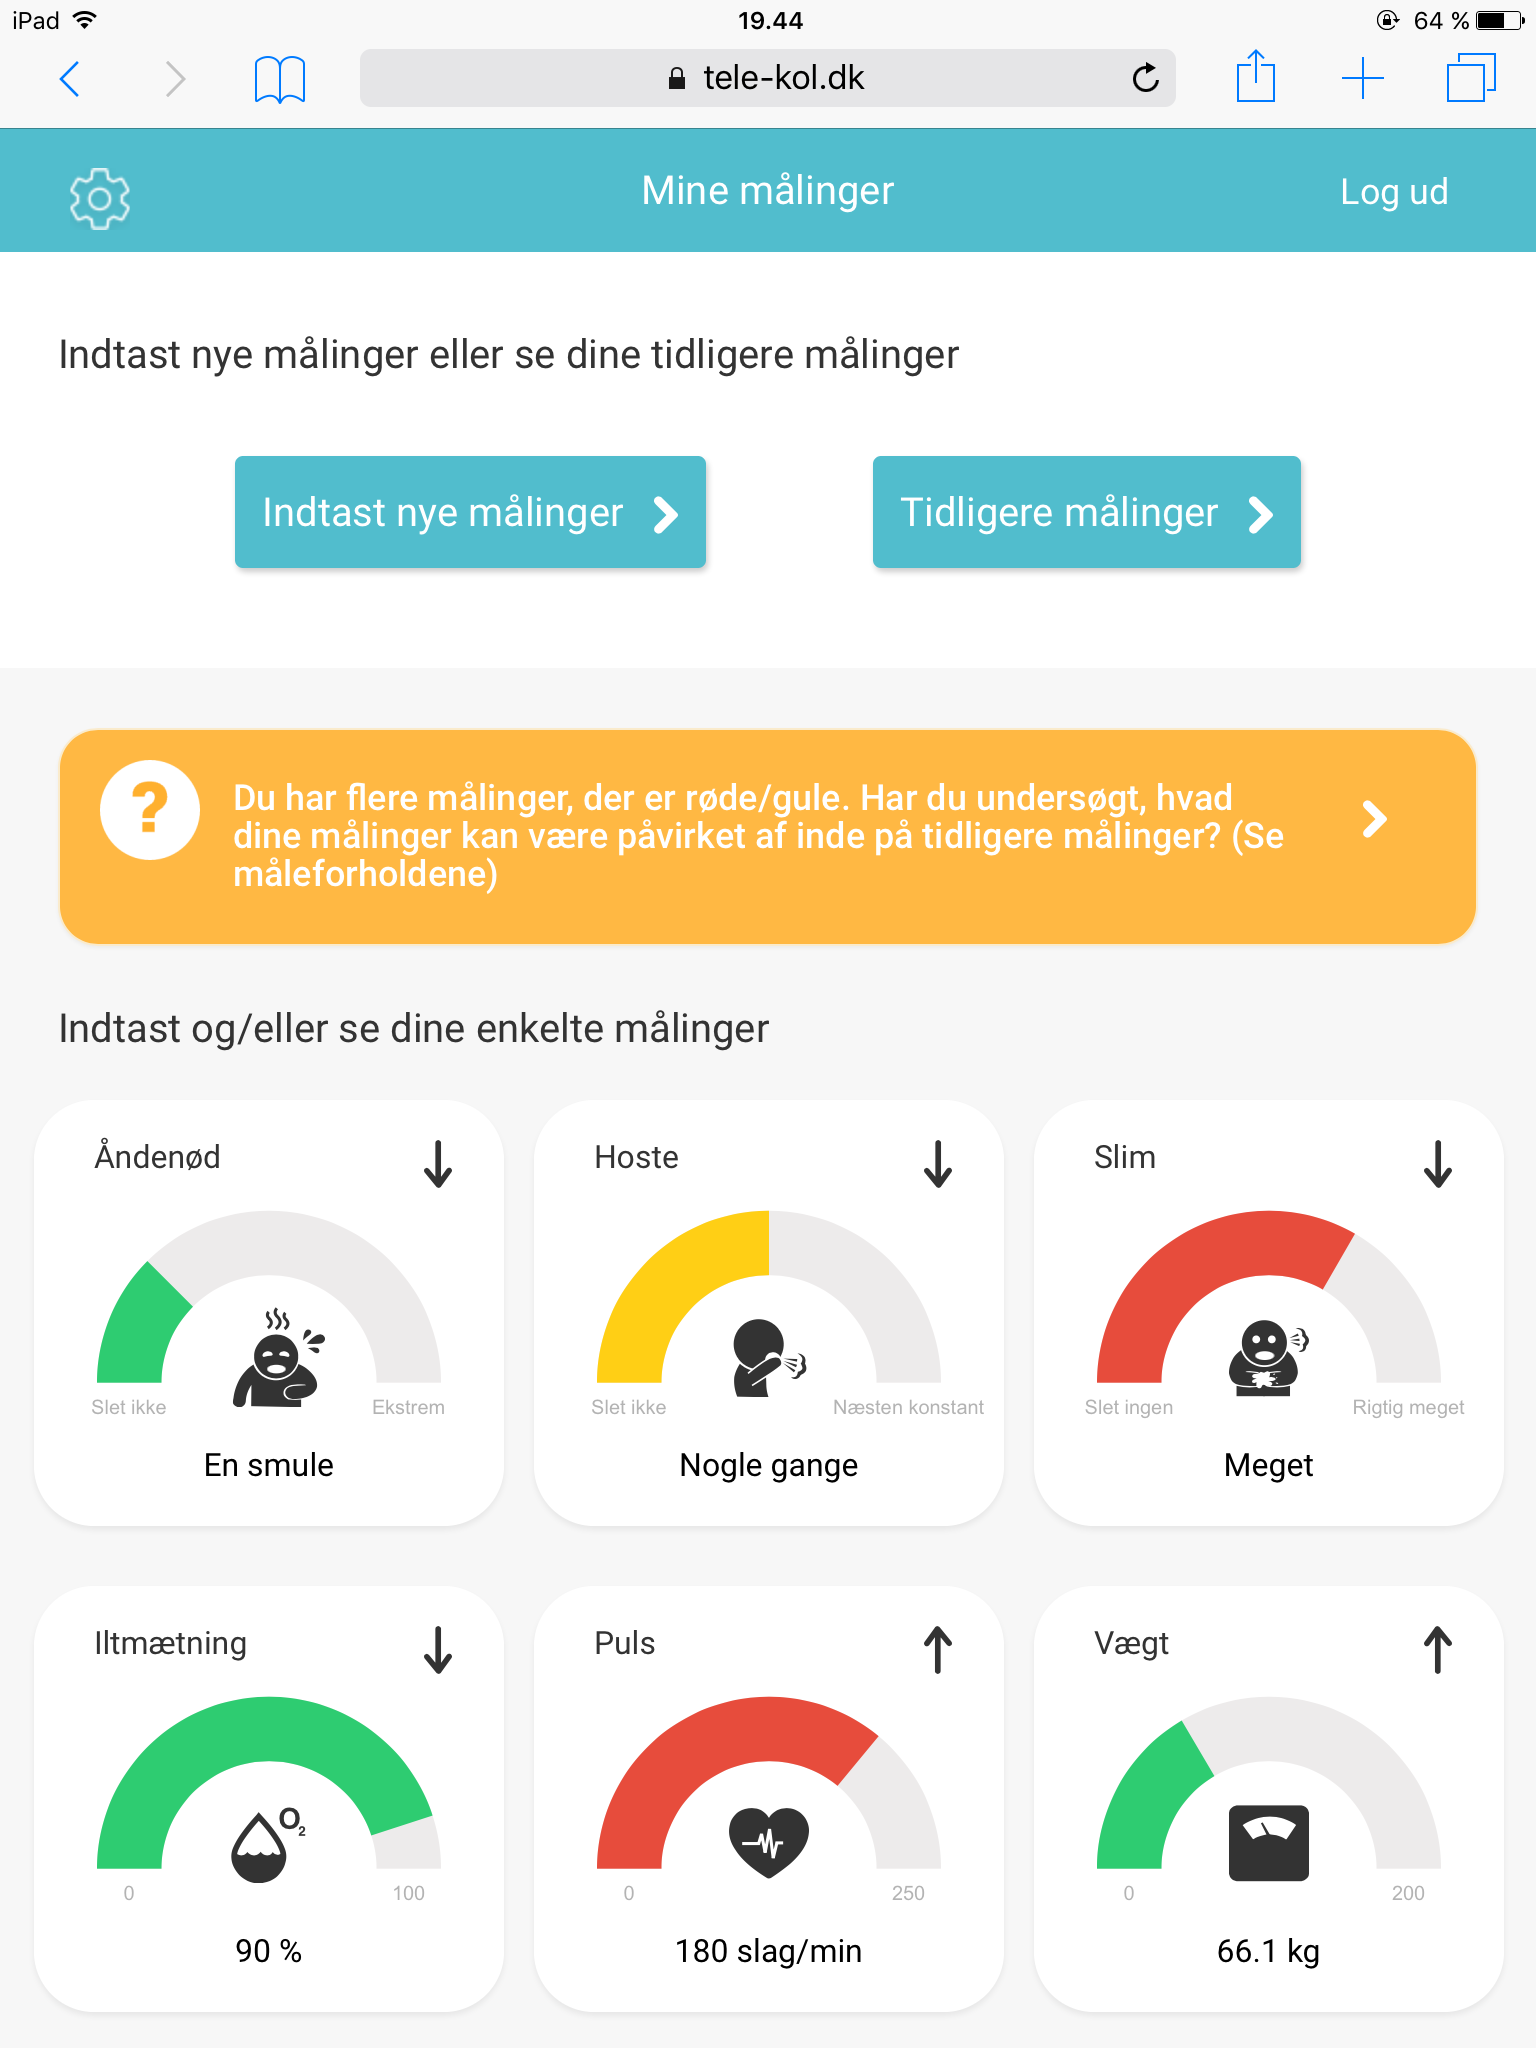
\includegraphics[width=\textwidth]{images/implementation/db.PNG}
    \caption{Redesigned dashboard}
    \label{fig:db2nd}
  \end{minipage}
\end{figure}

\subsection*{Reflective Questions}
Reflective questions were measure-specific in our first design proposal as seen on Figure \ref{fig:db1st}. We found in Study II that patients did not notice the reflective questions and thus decided to redesign the reflective questions as seen on Figure \ref{fig:db2nd}. 

Reflective questions were redesigned to target overall health status and updated depending on following conditions: 
 
\paragraph{When all color indicators were green (or only one yellow/red)}
\begin{itemize}
\item When should you be extra aware of your symptoms?
\item What is the status on your measures?
\item Is there any improvement in your latest measures? (Look at the arrows on each measure)
\item Have you explored what your measures might have been affected by in previous measures? (See measurement conditions)
\item Have you examined whether your normal range is adjusted to your needs? (Look at settings gear in the upper left corner)
\end{itemize}

\paragraph{When at least two measures were yellow/red}
\begin{itemize}
\item (You have multiple measures showing red/yellow.) Have you previously been able to improve your measures? How? 
\item (You have multiple measures showing red/yellow.) Which measures should you be aware of?
\item (You have multiple measures showing red/yellow.) How are your responses when you feel well?
\item You have multiple measures showing red/yellow. How long have your measures been like this? Is there anything you should be aware of?
\item You have multiple measures showing red/yellow. Is there any improvement in your latest measures? (Look at the arrows on each measure)
\item You have multiple measures showing red/yellow. Have you explored what your measures might have been affected by in previous measures? (See measurement conditions)
\item You have multiple measures showing red/yellow. Have you examined whether your normal range is adjusted to your needs? (Look at settings gear in the upper left corner)
\end{itemize}

The reflective question updates after one or more measures are  entered.

\subsection*{Visualisation Choice}
We provided patients with four visualisations in study II and from the feedback found that patients had different preferences. Based on findings from literature and patients' statements about the visualisations, we chose Visualisation 1 for long-term reflection (See Figure \ref{fig:visualization}). 
 
\subsection*{Normal Area}
Based on findings from previous research and findings from Study I showing that patients preferred their own normal area we provided the patients with a settings option to individualize the normal area for each objective measure (See Figure \ref{fig:settings}). 

\begin{figure}[h]
  \centering
  \begin{minipage}[b]{0.45\textwidth}
    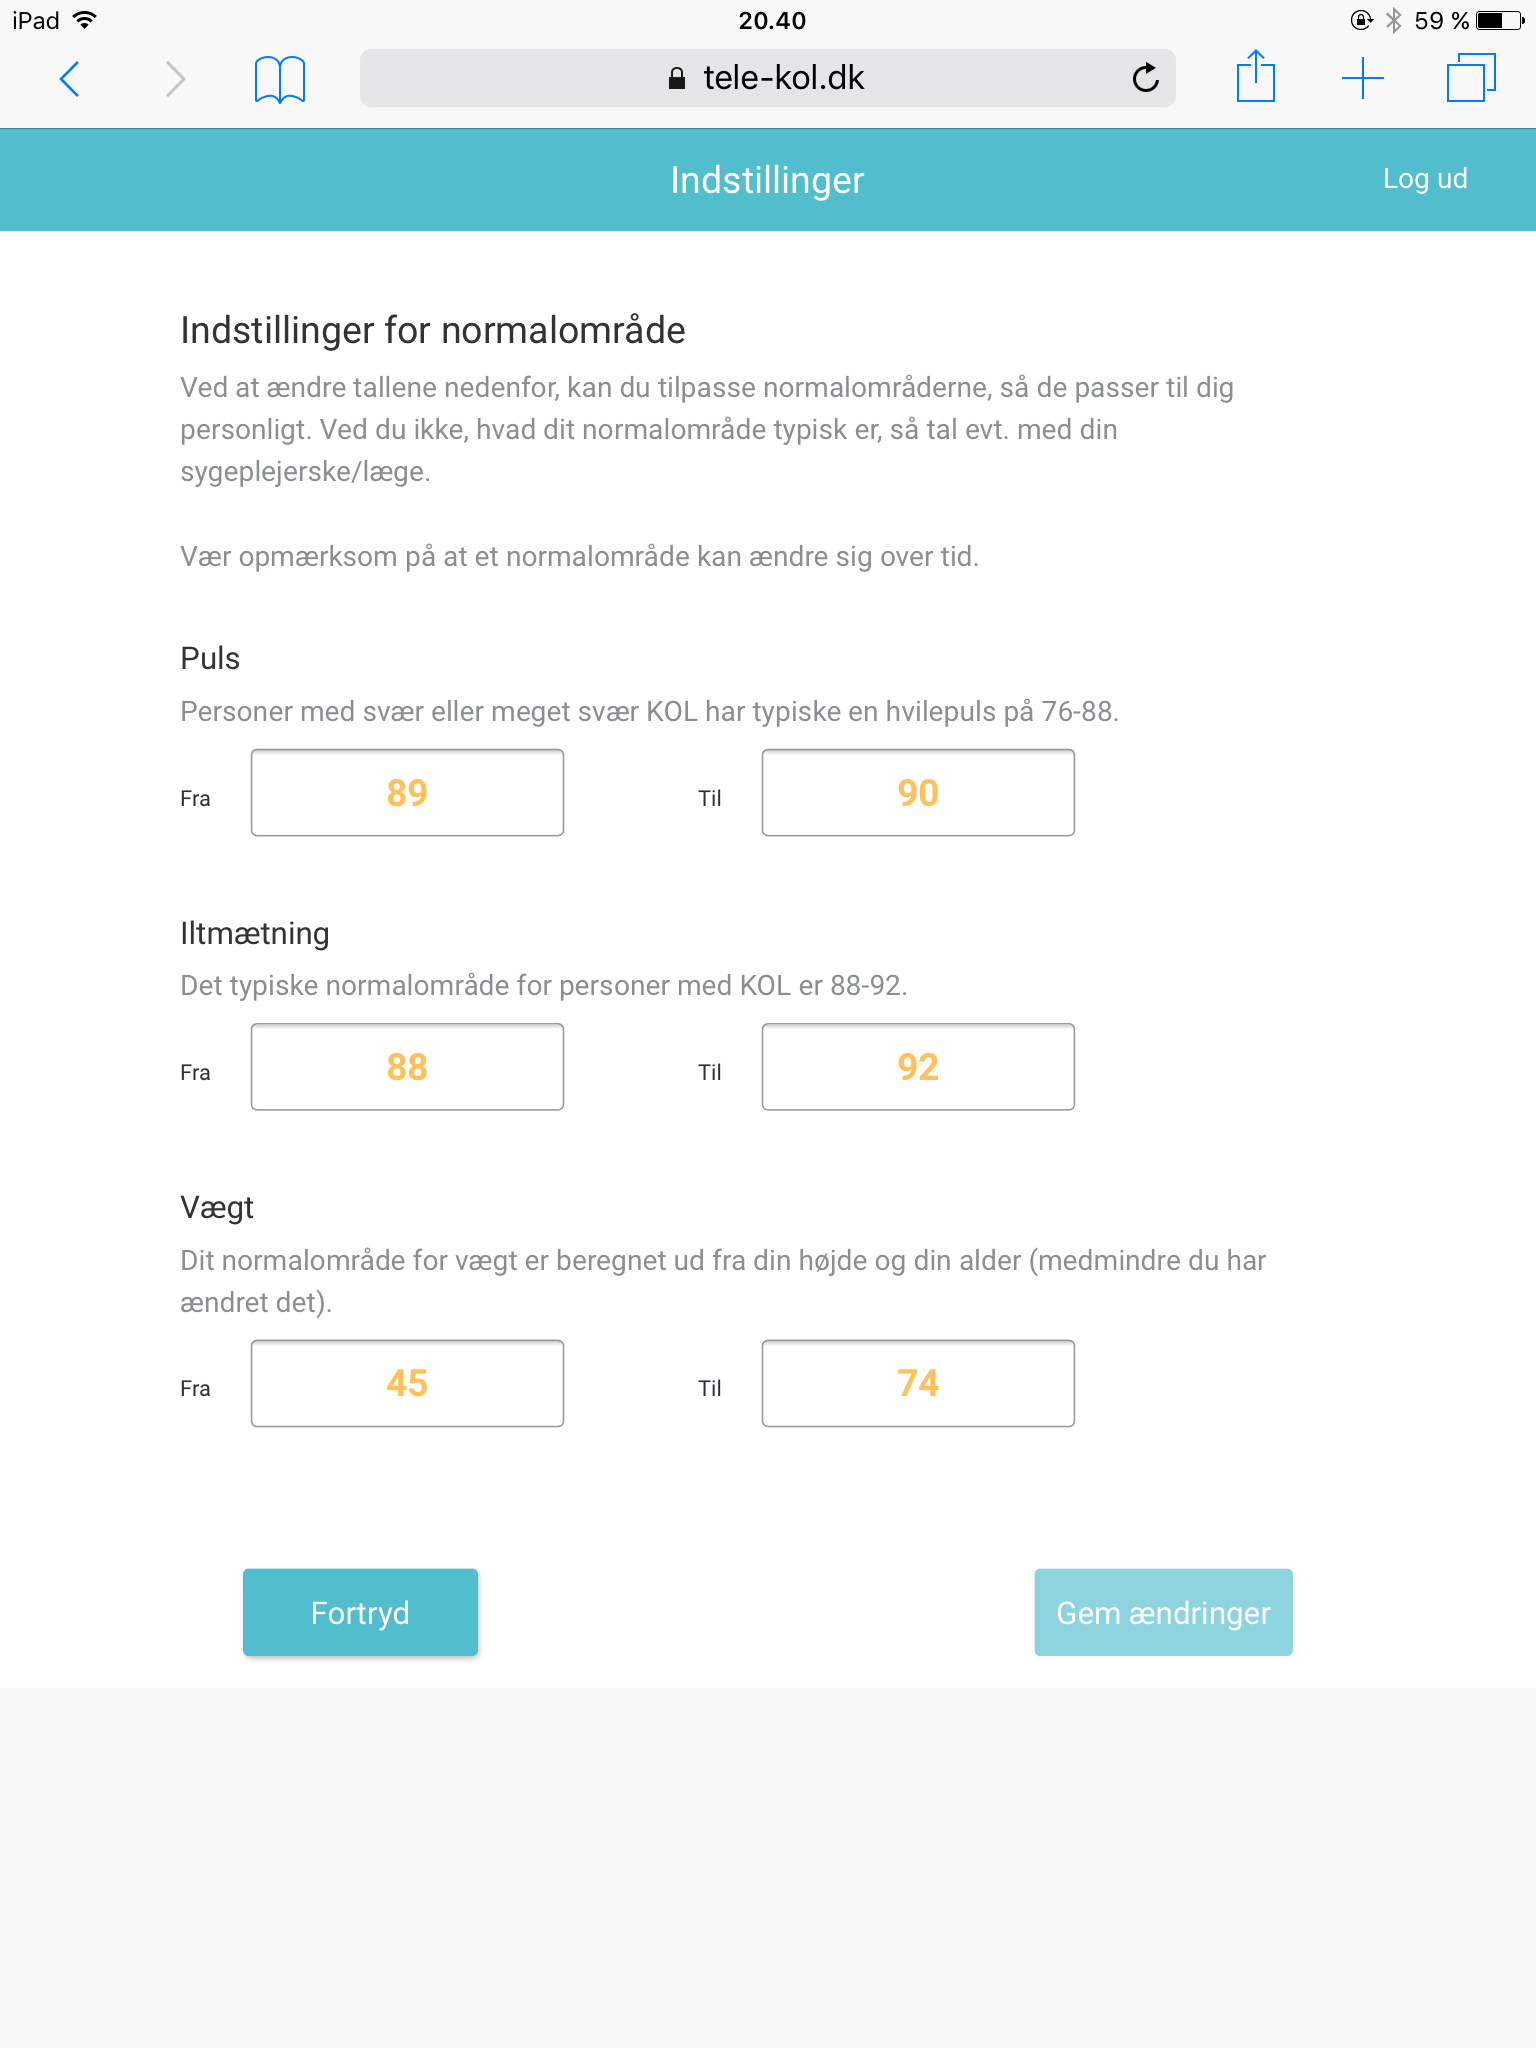
\includegraphics[width=\textwidth]{images/implementation/settingsImp.png}
    \caption{Settings.}
    \label{fig:settings}
  \end{minipage}
  \hfill
  \begin{minipage}[b]{0.45\textwidth}
    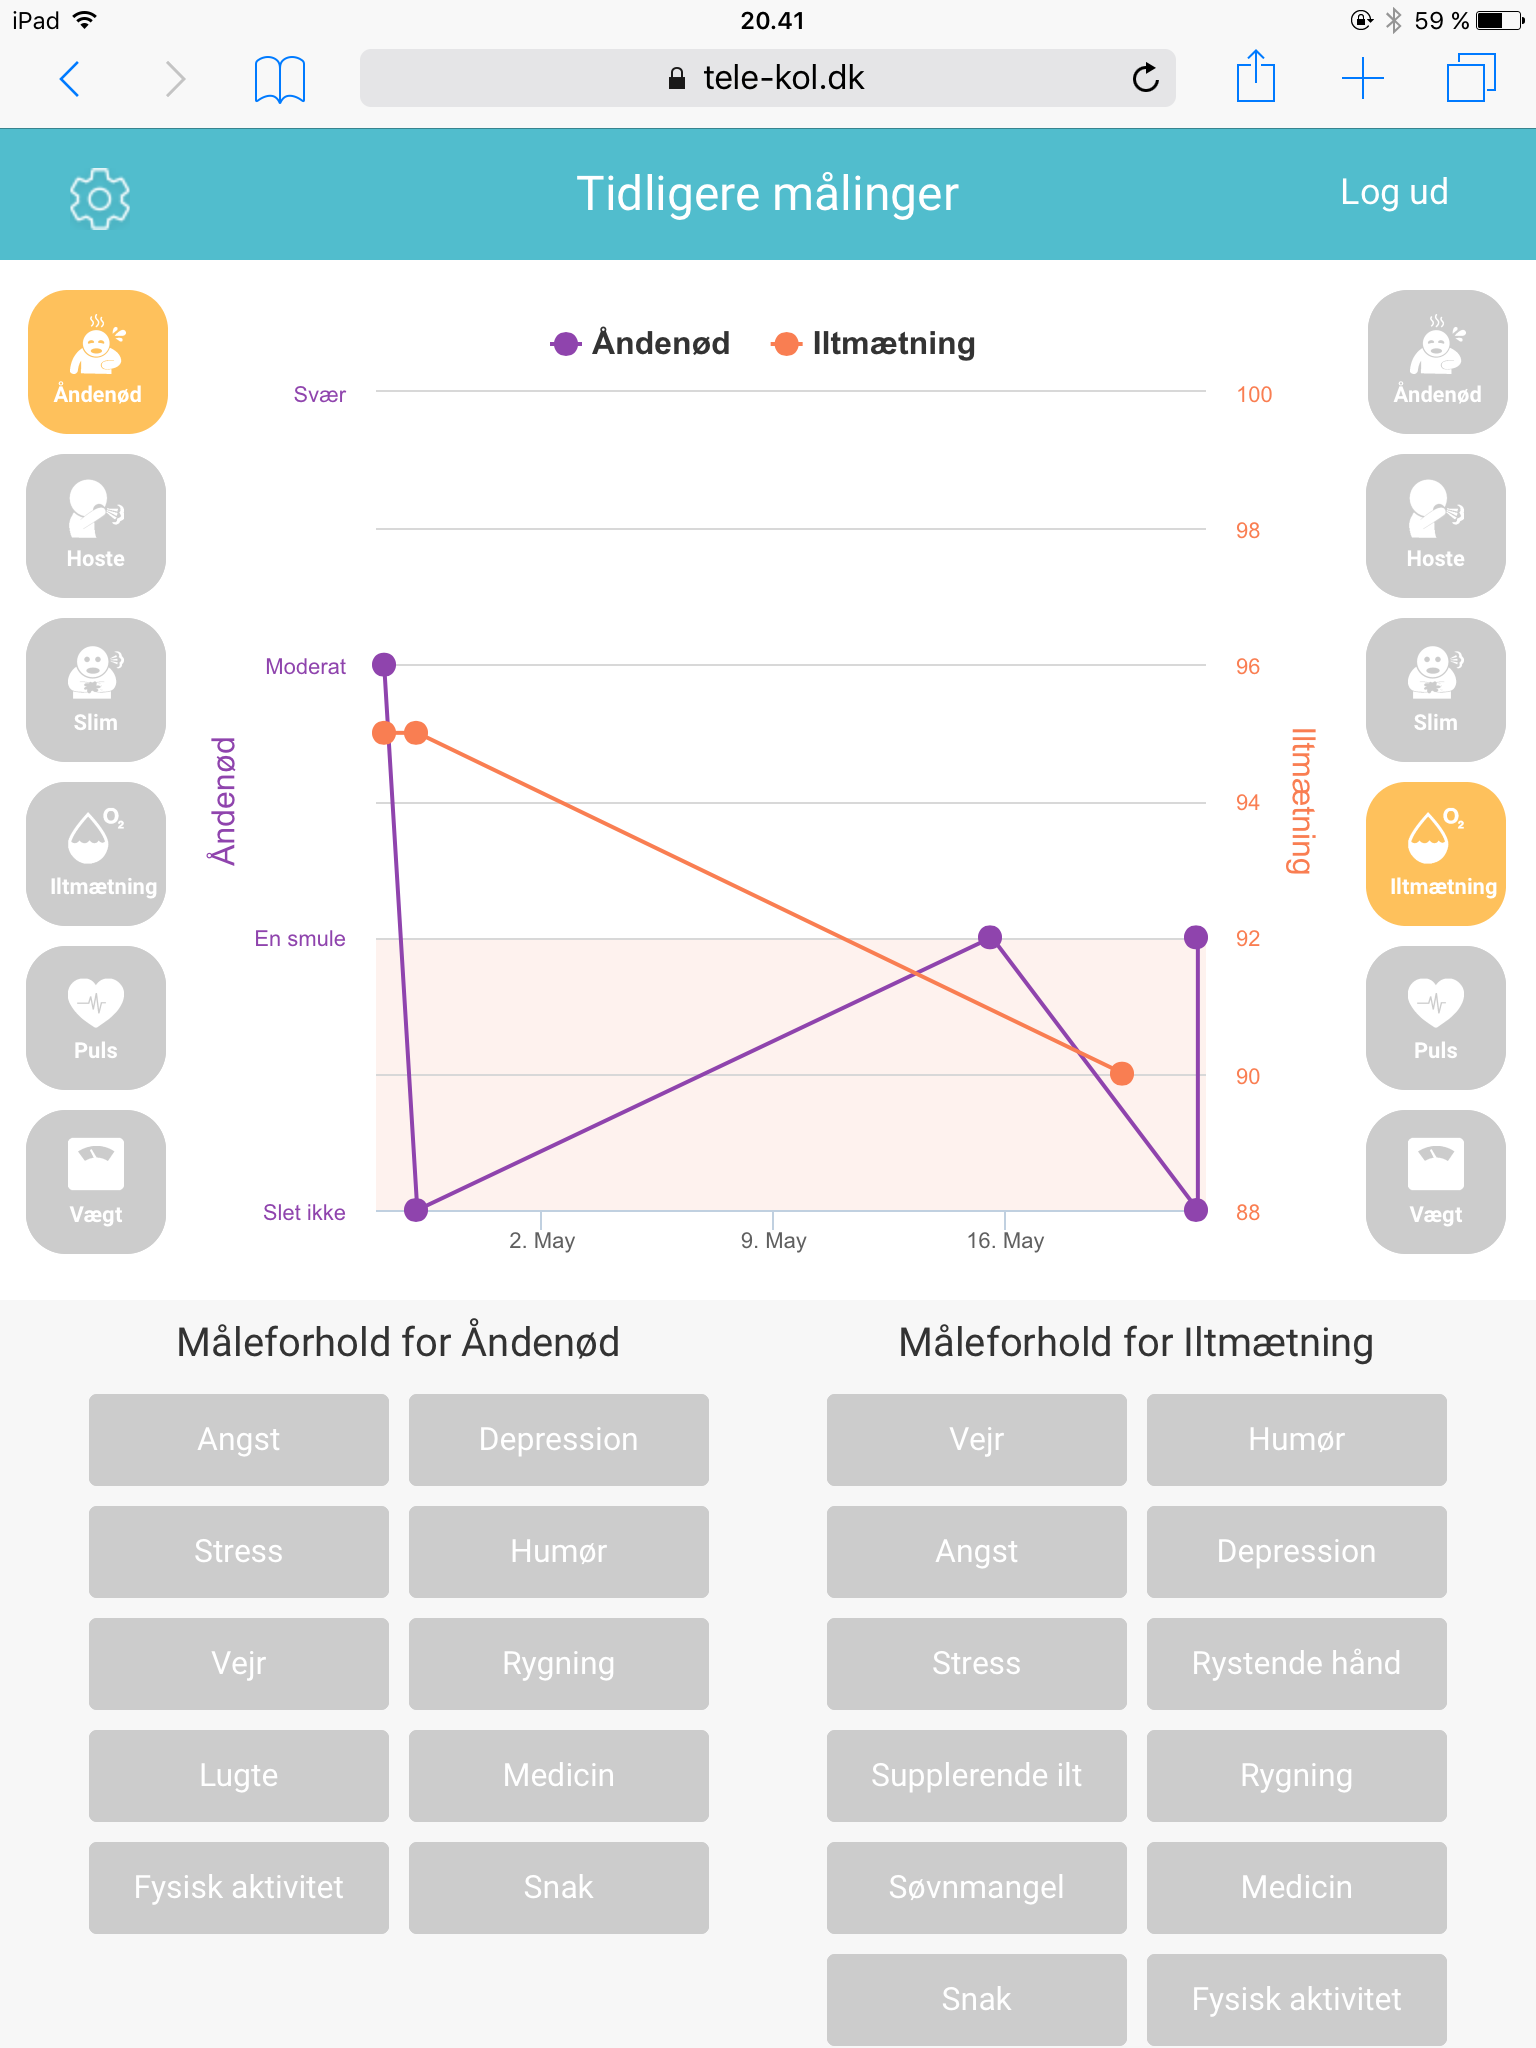
\includegraphics[width=\textwidth]{images/implementation/v1Imp.PNG}
    \caption{Visualisation 1.}
    \label{fig:visualization}
  \end{minipage}
\end{figure}

\section{Server-side Programming}
We used PHP to create sessions and to manipulate the user's data on the server-side. 

\subsection{Session}
We created a session, when the user logged into the system. A session is a way to store variables across multiple pages, which is the case (e.g.) when a patient navigates from the dashboard to collection. By saving an identification variable in the session, the system knows, who logged in across multiple pages. We programmed the session to automatically end after an hour. We created two types of directories, one for the patients and one for administration purposes. The administrator directory was made inaccessible to users (using the session).

\textbf{Administrator Access}

The administrator page provided access to our log, where we had a live view of the current use. We used it as investigation tool when we had a minor mix-up with user credentials and to see if patients had started using the system (in case any patients needed a reminder). We also made it possible to do manual logging, which we used when logging in as a patient.

We also made an administrator page for adding data to the different user's profiles, which we used when we entered the patients' measures from the paper template, which they filled out prior to the study. We also used it to add patient information to each user profile, where the system automatically calculated normal areas for weight. 


\subsection{Data}
We stored the patients' data in JSON, which is easy to navigate within when working client-side (in JavaScript). We developed a data-structure (See Figure \ref{fig:dStructure}). The data structure holds information of the user's normal areas, the measures, whether latest entry was all measures or just one (which decides if a reflection note will be stored on a single measure or on all six) and a reflection part that hold information of what reflective questions the user has received and the latest reflective question (in order to visualise it again when a user returns to the system).

\begin{figure}[h]
\centering
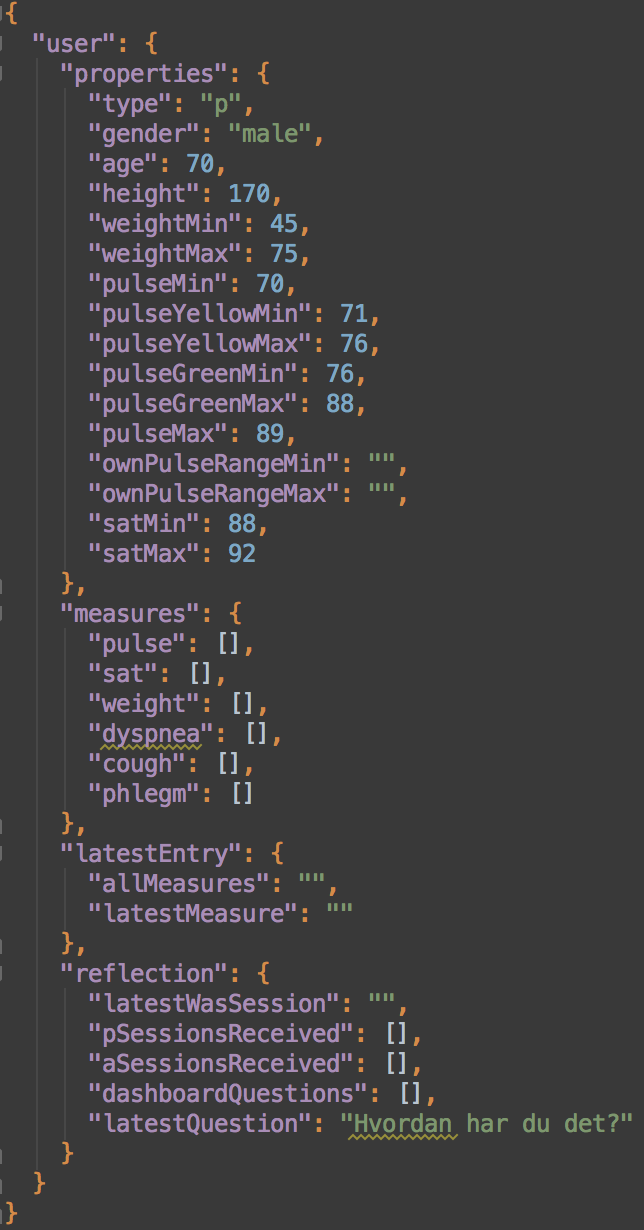
\includegraphics[scale=0.5]{images/implementation/dataStructure.png}
\caption{Data structure.}
\label{fig:dStructure}
\end{figure}

\textbf{Webservices}

We made multiple webservices to manipulate the user's data. With use of an example, we explain the principles of the webservices and how they are used to manipulate data. As an example we will save the latest reflective question the user has received in the user's data:

The server gets a call from the client with the latest reflective question received. By using a data class (which we developed for all webservices that manipulates user data) the data class, based on the session, finds the path to the user's JSON and returns the user data. The webservice now updates the data and saves it using the same data class again. The process can be seen on Figure \ref{fig:webservice}.

\begin{figure}[h]
\centering
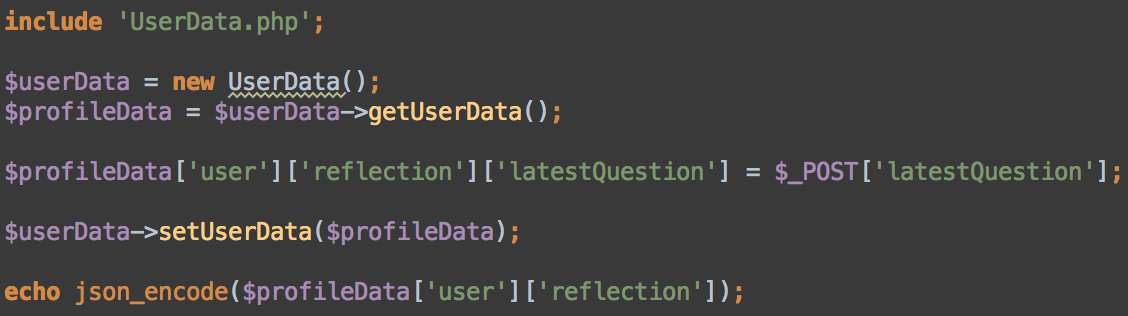
\includegraphics[scale=0.5]{images/implementation/webservice.png}
\caption{Webservice for saving the latest reflective question the user received.}
\label{fig:webservice}
\end{figure}
 
\section{Client-side}

\textbf{Get user data}

In order to get each user's data on login, we used ajax from the jQuery library. By updating HTML elements with use of jQuery we provide the user with visualisations matching the measures entered.

When wanting to add a line in the log (which is a simple .txt file), we called the server using ajax and sent the needed information (to log), whereafter the server added a line to the log (the server knows from the session who made the call).


\textbf{User Interface Elements}

The interface was built on the Bootstrap front-end framework \citep{bootstrap}. Bootstrap is open-source and provides HTML and CSS templates along with JavaScript components to design and build responsive web applications. For dashboard gauges we made use of the JavaScript plugin \textit{JustGage} \citep{justgage}, while we used \textit{Highcharts JS} \citep{highcharts} for visualising history data. 

Figure \ref{fig:gage} shows an example of creating the gauge for cough with parameters customized for each measure (number of options for the value, colors depending on current value, min and max text labels) 

\begin{figure}[h]
\centering
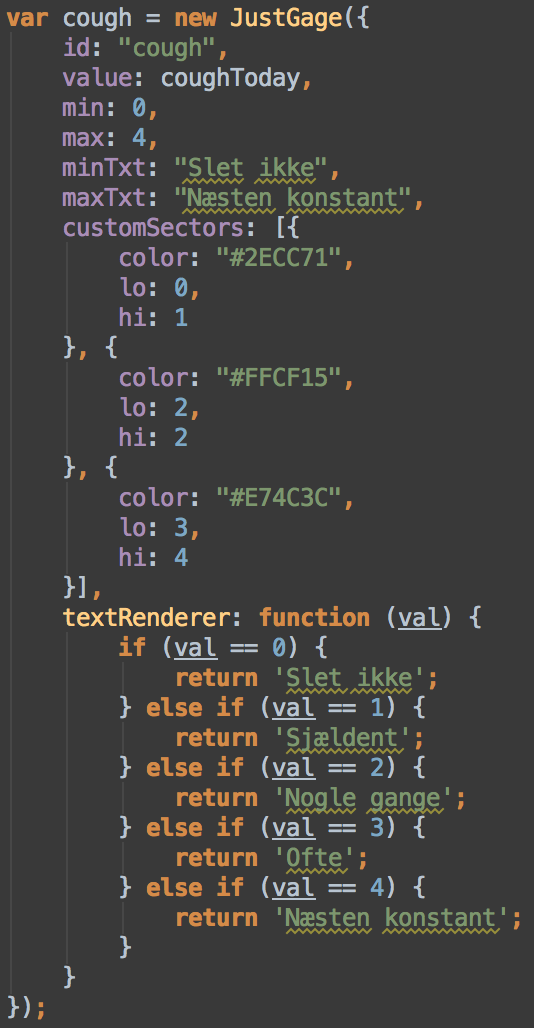
\includegraphics[scale=0.5]{images/implementation/gage.png}
\caption{Javascript code for creating a gage. In this case for cough.}
\label{fig:gage}
\end{figure}

 
\section{Security}
As we were working with patients' data, we had an ethical responsibility. We handled all the patients' data anonymously, such that no patient could be identified from the data on the server.

In principle this should be sufficient, but we added additional security to the system, which we consider as good practice. First of all we used a SSL certificate to keep sensitive information encrypted, when the user sent data to the server. This made sniffing of data less easy. Since we used JSON files on the server to store patient data, we also restricted the access to the JSON files with use of .htaccess files and .htpasswd files thus when trying to access the files a username and a password is needed, in order to get access to that directory on the server. This system is not at all considered as a highly secure website, but sufficient for a two week trial trial. A database setup would be a good consideration for future use.